\documentclass[12pt]{article}

\usepackage[margin=50pt]{geometry}
\usepackage{amsmath}
\usepackage{amssymb}
\usepackage{graphicx}
\usepackage{braket}
\usepackage{mathtools}
\usepackage{enumitem}

\graphicspath{/images}
\geometry{footskip=0.8cm}

\title{Introduction to Quantum Computing}
\author{Thomas Vroom}

\begin{document}
\maketitle

%
% Lecture 1 - Introdution.
%
\section*{Lecture 1 - Introduction}
The \textbf{Church-Turing thesis} states that anything that is computable, can be computed by an appropriate \textbf{Turing machine}.
It also states that efficient algorithm design is \textit{independent} of the underlying model of computation.
Classical computing (based on the Turing machine-model of computation) does not seem able to efficiently simulate quantum mechanics.

\begin{center}
    "The best way to simulate quantum mechanics, is to use quantum mechanics."
\end{center}

\noindent
To get a better understanding of the quantum computational process, we will first look at two classical physics experiments.

\subsection*{The Double-Slit Experiment}
The double-slit experiment demonstrates the wave-particle duality of light:

\begin{figure}[h]
    \centering
    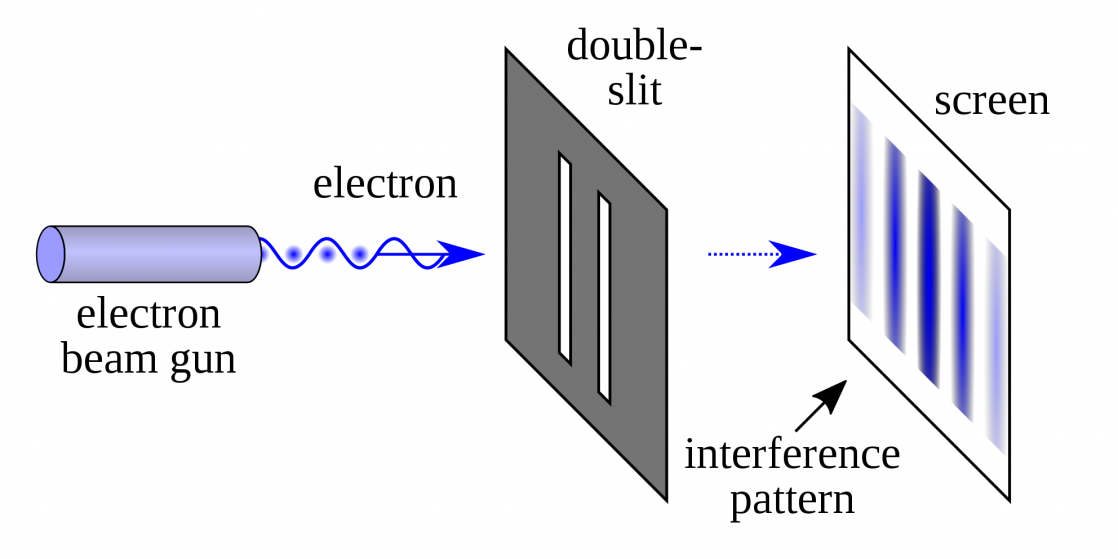
\includegraphics[scale=0.25]{images/double_slit_experiment.png}
\end{figure}

\noindent
Electrons fired at the screen can either undergo \textbf{constructive interference} (i.e. they add together) or \textbf{destructive interference} (i.e. they cancel out), meaning that the electrons behave like waves.

\newpage
\subsection*{The Stern-Gerlach Experiment}
The Stern-Gerlach experiment measures the spin of electrons:

\begin{figure}[h]
    \centering
    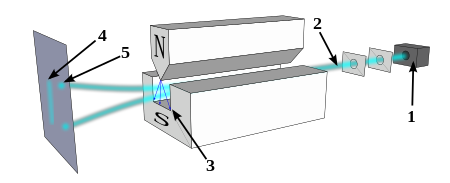
\includegraphics[scale=0.75]{images/stern_gerlach_experiment.png}
\end{figure}

\noindent
Atoms are fired through a magnetic field, causing them to split into an \textbf{upwards spin} or a \textbf{downwards spin}.
There is no in-between, even though classical physics predicts that there should be.
If we continue measuring the spin of the atoms, we will continue to get the same results.
If we rotate the apparatus by 90 degrees and measure all the previous "up spins", we will see that 50\% of them are deflected into one direction, while the other 50\% are deflected into the other direction, even though classical physics suggests that none should be deflected at all.

\subsection*{Qbits}
We can use the spin of an electron to create an elementary unit of quantum information, called a \textbf{Qbit}.
Similarly to a classical bit (Cbit), a Qbit can take values of either 0 (down spin) or 1 (up spin).
In addition to this, a Qbit can also be in a \textbf{superposition} of both:
\[ \ket{s} = \alpha \ket{\uparrow} + \beta \ket{\downarrow} \]

\noindent
Such that $\alpha^2 + \beta^2 = 1$.
When we look at the value of a Qbit that is in a superposition of two or more states, then its superposition \textbf{collapses} into exactly one of the states.
This intuitively means that, if we observe $s$, we expect to see a $\uparrow$ spin with probability $\alpha^2$ and a $\downarrow$ spin with probability $\beta^2$.
The numbers $\alpha$ and $\beta$ are called the \textbf{amplitudes} of the corresponding states, and can be any numbers (real, negative, complex, etc.).

\noindent
\\
If we were to replace $\alpha$ and $\beta$ in the above equation with $\alpha^2$ and $\beta^2$, then we do not allow the existence of negative amplitudes.
If we allow amplitudes to be negative, then we can get \textbf{destructive interference} between the two states, which is not possible if we only allow positive amplitudes.
This gives the Qbit a computational advantage over the Cbit.

\noindent
\\
Qbits can be distinguished from Cbits by the following properties:

\begin{itemize}
    \item \textbf{Superposition}.
    \item \textbf{Interference}.
    \item \textbf{Entanglement}.
\end{itemize}

\noindent
It is important to note that one Qbit can encode up to two classical bits of information.
Throughout this course we will see how these properties give rise to some powerful quantum algorithms.

%
% Lecture 2 - Qbits I.
%
\newpage
\section*{Lecture 2 - Qbits I}
During the S-G experiment, we saw that the spin of an electron, instead of being a continuous value, is actually quantized into either $\uparrow$ or $\downarrow$.
Before the experiment, the spin has an unknown orientation: it is in a superposition of both $\uparrow$ and $\downarrow$:
\[ \ket{\psi} = \alpha \ket{\uparrow} + \beta \ket{\downarrow} \]

\noindent
Such that $\alpha^2 + \beta^2 = 1$.
Observing the state of the electron constitutes as a \textbf{measurement}, which causes the superposition to collapse into exactly one of the two states (with corresponding probabilities $\alpha^2$ and $\beta^2$).
The act of measurement in a quantum state is irreversible.
Once we have observed a state, the particle will stay in that state no matter how many times we measure it again.

\noindent
\\
If we \textit{rotate} the apparatus by, for example, $90^{\circ}$, and we repeat the experiment, an electron that was previously measured $\ket{\uparrow}$, will be measured to have a 50\% chance to be measured in either of the two new directions.
By rotating the apparatus we induce a new \textbf{base of measurement}, with superposition:
\[ \ket{\psi} = \gamma \ket{\rightarrow} + \delta \ket{\leftarrow} \]

\noindent
Such that $\gamma^2 + \delta^2 = 1$.
So which superposition is the true superposition of $\ket{\psi}$?
It depends on what we are interested in (i.e. in which direction we are making the measurement).

\noindent
\\
Note that a superposition of basic states describes more than just the probabilities.
For example, take the superpositions:
\[ \frac{1}{\sqrt{2}} \ket{\uparrow} + \frac{1}{\sqrt{2}} \ket{\downarrow} \]
\[ \frac{1}{\sqrt{2}} \ket{\uparrow} - \frac{1}{\sqrt{2}} \ket{\downarrow} \]

\noindent
Both of these superpositions have the same probability of being on either state when we make a measurement, but they are very different superpositions.

\subsection*{Geometrical Representation}
We can encode the two states $\ket{\uparrow}$ and $\ket{\downarrow}$ as the following vectors:
\[ \ket{\uparrow} = \begin{pmatrix}
    1 \\
    0
\end{pmatrix}, \text{ i.e. } \alpha = 1, \beta = 0 \]
\[ \ket{\downarrow} = \begin{pmatrix}
    0 \\
    1
\end{pmatrix}, \text{ i.e. } \alpha = 0, \beta = 1 \]

\noindent
Vectors in quantum mechanics are often denoted in \textbf{Dirac notation}.
Here the vector $\ket{.}$ is called a \textbf{ket} (column vector) and the vector $\bra{.}$ is called a \textbf{bra} (row vector).

\noindent
\\
Using the above-mentioned vectors as basis, we can represent any superposition of $\ket{\uparrow}$ and $\ket{\downarrow}$ as a \textbf{linear combination}:

\newpage
\begin{figure}[h]
    \centering
    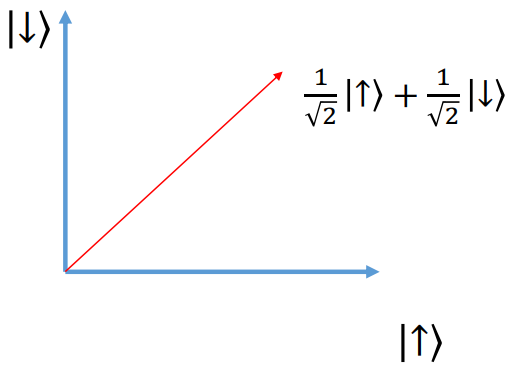
\includegraphics[scale=0.65]{images/geometrical_representation_1.PNG}
\end{figure}

\noindent
We can also think of a Qbit as a \textbf{unit-vector} which makes an angle $\theta$ with the $\ket{\uparrow}$ vector:
\[ \ket{\psi} = \cos \theta \ket{\uparrow} + \sin \theta \ket{\downarrow} \]

\noindent
If we measure this Qbit, we observe $\ket{\uparrow}$ with a probability of $\cos^2 \theta$ and $\ket{\downarrow}$ with a probability of $\sin^2 \theta = \cos^2 \left( \frac{\pi}{2} - \theta \right)$.
This shows that a measurement is simply a \textbf{projection} onto the standard basis vectors (with corresponding probabilities).

\noindent
\\
Say we want to measure the Qbit in a different basis, for example:

\begin{figure}[h]
    \centering
    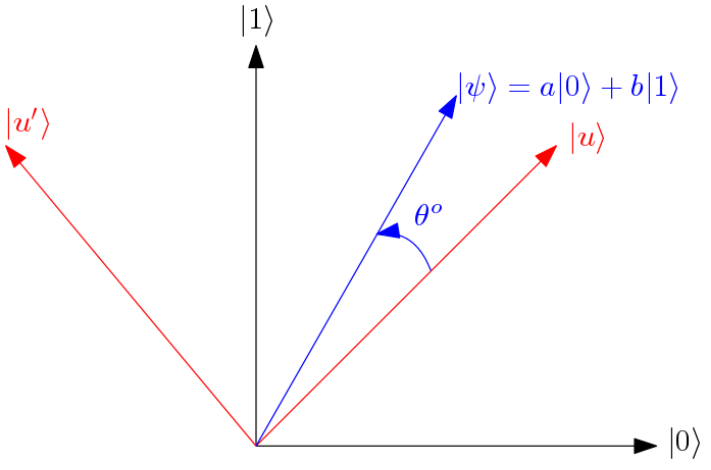
\includegraphics[scale=0.65]{images/geometrical_representation_2.PNG}
\end{figure}

\noindent
Here we are interested in measuring the Qbit $\ket{\psi}$ in the new basis $\{ u, u^\prime \}$.
We expect to observe $\ket{u}$ with probability $\cos^2 \theta$ and $\ket{u^\prime}$ with probability $\sin^2 \theta$.
Since $\ket{u}$ and $\ket{u^\prime}$ are both superpositions of $\ket{0}$ and $\ket{1}$, we can write them as:
\[ \ket{u} = \frac{1}{\sqrt{2}} \ket{0} + \frac{1}{\sqrt{2}} \ket{1} \]
\[ \ket{u^\prime} = -\frac{1}{\sqrt{2}} \ket{0} + \frac{1}{\sqrt{2}} \ket{1} \]

\noindent
Measuring Qbits in the basis $\{ u, u^\prime \}$ means that we are not interested anymore in the $\ket{0}$ and $\ket{1}$ states, but rather in the $\ket{u}$ and $\ket{u^\prime}$ states.

\newpage
\subsection*{Linear Algebra in Dirac Notation}
Remember how a ket is a column vector and a bra is a row vector, for example:
\[ \ket{\phi_1} = \begin{pmatrix}
    1 \\
    2
\end{pmatrix} \]
\[ \bra{\phi_2} = \begin{pmatrix}
    3 & 4
\end{pmatrix} = \begin{pmatrix}
    3 \\
    4
\end{pmatrix}^T \]

\noindent
If $\ket{a} = \begin{pmatrix}
    a_1 \\
    a_2
\end{pmatrix}$ and $\ket{b} = \begin{pmatrix}
    b_1 \\
    b_2
\end{pmatrix}$, then $\ket{a + b} = \begin{pmatrix}
    a_1 + b_1 \\
    a_2 + b_2
\end{pmatrix} = \ket{b + a}$.

\noindent
\\
The \textbf{inner (dot) product} between a bra and a ket is defined as:
\[ \braket{a | b} = a^T b = a_1b_1 + a_2b_2 \]

\noindent
The length of a ket can be calculated as:
\[ \left\lvert \ket{a} \right\rvert = \sqrt{\sum_{i} a_i^2} = \sqrt{\braket{a | a}} \]

\noindent
We will mostly be dealing with \textbf{unit-vectors} (length = 1).

\noindent
\\
Two kets $\ket{a}$, $\ket{b}$ are \textbf{orthogonal} if and only if $\braket{a | b} = 0$.

\noindent
\\
An $n$-dimensional \textbf{orthonormal basis} is a collection of $n$ unit-vectors that are all orthogonal to each other.
For example, in a 2-dimensional space, we need two vectors $\ket{a}$ and $\ket{b}$ such that:
\begin{table}[h]
    \centering
    \begin{tabular}{rcl}
    $\braket{a | a}$ & $=$ & 1  \\
    $\braket{b | b}$ & $=$ & 1 \\
    $\braket{a | b}$ & $=$ & 0
    \end{tabular}
\end{table}

\noindent
Let $\ket{v}$ be an $n$-dimensional ket, and $\{ \ket{b_1}, \ket{b_2}, ... , \ket{b_n} \}$ is a basis for $\mathbb{R}^n$. 
We want to write $\ket{v}$ as a \textbf{linear combination} of the basis vectors, i.e. $\ket{v} = w_1\ket{b_1} + w_2\ket{b_2} + ... + w_n\ket{b_n}$.
We can show that $w_i = \braket{b_i | v}$, and thus $\ket{v} = \braket{b_1 | v}\ket{b_1} + \braket{b_2 | v}\ket{b_2} + ... + \braket{b_n | v}\ket{b_n}$.

\noindent
\\
To describe the evolution of a quantum system, we also consider a third form of multiplication on matrices, the \textbf{tensor product}.
Let $A$ and $B$ be two matrices of any dimension, then the tensor product $A \otimes B$ is defined as:
\[ A \otimes B = \begin{bmatrix*}[c]
    a_{11}B \ \dots \ a_{1m}B \\
    \vdots \ \ddots \ \vdots \\
    a_{n1}B \ \dots \ a_{nm}B
\end{bmatrix*} \]

\noindent
When tensor-multiplying kets, the notation is as follows:
\[ \ket{\psi} \otimes \ket{\phi} = \ket{\psi}\ket{\phi} = \ket{\psi\phi} \]

\noindent
Note that tensor-multiplication is \textbf{associative} (i.e. $a \otimes (b \otimes c) = (a \otimes b) \otimes c$).

%
% Lecture 3 - Qbits II.
%
\newpage
\section*{Lecture 3 - Qbits II}
The orthonormal basis corresponding to measuring the spin in the vertical direction is given by:
\[ \ket{\uparrow} = \begin{pmatrix}
    1 \\
    0
\end{pmatrix}, \ket{\downarrow} = \begin{pmatrix}
    0 \\
    1
\end{pmatrix} \]

\noindent
The orthonormal basis corresponding to measuring the spin in the horizontal direction is given by:
\[ \ket{\rightarrow} = \begin{pmatrix}
    \frac{1}{\sqrt{2}} \\
    \frac{-1}{\sqrt{2}}
\end{pmatrix}, \ket{\leftarrow} = \begin{pmatrix}
    \frac{1}{\sqrt{2}} \\
    \frac{1}{\sqrt{2}}
\end{pmatrix} \]

\noindent
Let us start with measuring the spin in the vertical direction:
\[ \ket{\psi} = \alpha \ket{\uparrow} + \beta \ket{\downarrow} \]

\noindent
If we measure the spin to be $\ket{\uparrow}$, the new state is:
\[ \ket{\psi} = 1 \cdot \ket{\uparrow} + 0 \cdot \ket{\downarrow} \]

\noindent
If we keep measuring $\ket{\psi}$ in the vertical direction, we will keep getting $\ket{\uparrow}$ with probability 1.
What will happen if we measure the spin of $\ket{\psi}$ in the horizontal direction?
To do that, we must first write $\ket{\psi} = \ket{\uparrow}$ in terms of the horizontal basis (i.e. we need to find $\gamma, \delta$ such that $\gamma^2 + \delta^2 = 1$ and $\ket{\psi} = \gamma \ket{\rightarrow} + \delta \ket{\leftarrow}$).
First, we construct the transformation matrix $H$ that corresponds to the horizontal basis:
\[ H = \begin{pmatrix}
    \frac{1}{\sqrt{2}} & \frac{1}{\sqrt{2}} \\
    \frac{-1}{\sqrt{2}} & \frac{1}{\sqrt{2}}
\end{pmatrix} \]

\noindent
Now, we can multiply $H^T$ with $\ket{\psi}$ to get the new probability amplitudes with respect to the horizontal axis:
\[ \begin{pmatrix}
    \frac{1}{\sqrt{2}} & \frac{-1}{\sqrt{2}} \\
    \frac{1}{\sqrt{2}} & \frac{1}{\sqrt{2}}
\end{pmatrix} \begin{pmatrix}
    1 \\
    0
\end{pmatrix} = \begin{pmatrix}
    \frac{1}{\sqrt{2}} \\
    \frac{1}{\sqrt{2}}
\end{pmatrix} \]

\noindent
This gives:
\[ \ket{\psi} = \frac{1}{\sqrt{2}}\ket{\rightarrow} + \frac{1}{\sqrt{2}}\ket{\leftarrow} \]

\noindent
So, when we measure $\ket{\psi} = \ket{\uparrow}$ in the horizontal direction, we get that the electron is deflected either in the left or the right direction, each with probability $\frac{1}{2}$.

\subsection*{Equivalent States}
Consider the following two superpositions:
\[ \ket{\psi_1} = \frac{1}{\sqrt{2}}\ket{\uparrow} + \frac{1}{\sqrt{2}}\ket{\downarrow} \]
\[ \ket{\psi_2} = -\frac{1}{\sqrt{2}}\ket{\uparrow} - \frac{1}{\sqrt{2}}\ket{\downarrow} \]

\noindent
Both of these superpositions have the same probability of being measured in either $\ket{\uparrow}$ or $\ket{\downarrow}$.
Is there an experiment (i.e. measurement) we can perform that would allow us to distinguish between these two superpositions?

\newpage
\noindent
Suppose we make the measurement in some other basis $\{ \ket{u_1}, \ket{u_2} \}$.
To get the probabilities for this basis, we need to write $\ket{\uparrow}$ and $\ket{\downarrow}$ in terms of $\ket{u_1}$ and $\ket{u_2}$:
\[ \ket{\uparrow} = \alpha \ket{u_1} + \beta \ket{u_2} \]
\[ \ket{\downarrow} = \gamma \ket{u_1} + \delta \ket{u_2} \]

\noindent
This gives:
\[ \ket{\psi_1} = \frac{\alpha + \gamma}{\sqrt{2}}\ket{u_1} + \frac{\beta + \delta}{\sqrt{2}}\ket{u_2} \]
\[ \ket{\psi_2} = -\frac{\alpha + \gamma}{\sqrt{2}}\ket{u_1} - \frac{\beta + \delta}{\sqrt{2}}\ket{u_2} \]

\noindent
In both cases, we still get identical probabilities.
This means that there is no experiment we can perform to distinguish between these two superpositions.
We call $\ket{\psi_1}$ and $\ket{\psi_2}$ \textbf{indistinguishable}.

\subsection*{Photon Polarization}
A photon is an electromagnetic wave that oscillates in a certain axis.
The \textbf{polarization} of a photon is the direction of the electric field (vertically or horizontally orientated).
We can change the polarization of a photon by applying a \textbf{polaroid filter}:

\begin{figure}[h]
    \centering
    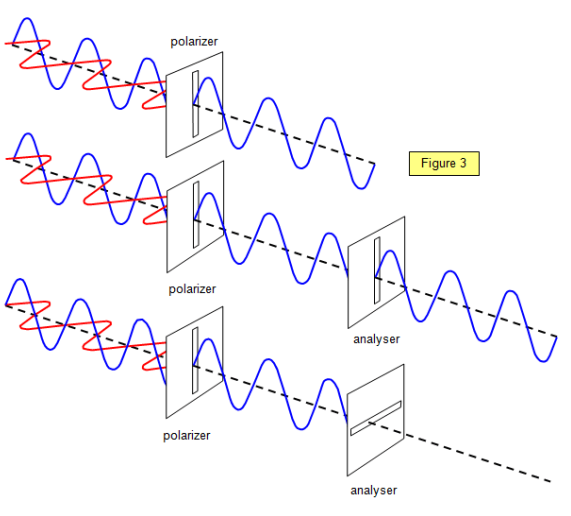
\includegraphics[scale=0.75]{images/photon_polarization_1.PNG}
\end{figure}

\noindent
Note that the horizontally polarized photons cannot pass through the vertical polaroid, and vice versa.
Logically, no single photon is able to pass through a vertical polaroid followed by a horizontal polaroid, and vice versa.

\noindent
\\
Assume we denote the horizontal polarization by the state $\ket{0}$ and the vertical polarization by the state $\ket{1}$.
If a photon makes a $45^\circ$ angle between the horizontal and vertical polarization axes, then its state can be described as the following superposition:
\[ \ket{\psi} = \frac{1}{\sqrt{2}}\ket{0} + \frac{1}{\sqrt{2}}\ket{1} \]

\newpage
\noindent
This superposition shows that a photon with polarization of $45^\circ$ will pass through a horizontal / vertical polaroid with probability $\frac{1}{2}$.

\noindent
\\
Assume our photon has polarization $\ket{\psi} = \cos \theta \ket{\uparrow} + \sin \theta \ket{\rightarrow}$, and that we have the following setup:

\begin{enumerate}
    \item A vertical polaroid.
    \item A polaroid at $45^\circ$.
    \item A horizontal polaroid.
\end{enumerate}

\noindent
We can calculate the probability of the photon passing through each polaroid as follows:

\begin{enumerate}
    \item The probability of the photon passing through the first polaroid is $\cos^2 \theta$.
    Its new state is $\ket{\psi} = \ket{\uparrow}$ (only vertically polarized photons have made it through).
    \item The probability of the photon passing through the second polaroid is $\frac{1}{2}$.
    If it makes it through the second polaroid, its new state is $\ket{\psi} = \frac{1}{\sqrt{2}}\ket{\uparrow} + \frac{1}{\sqrt{2}}\ket{\rightarrow}$.
    \item The probability of the photon passing through the third polaroid is $\frac{1}{2}$.
    This means that the probability of the photon making it through all three polaroids is $\frac{1}{2} \cdot \frac{1}{2} = \frac{1}{4}$ (we assume it already made it through the first one).
\end{enumerate}

\noindent
Note that without the diagonal polaroid, it is impossible to get a photon through the vertical and horizontal polaroids.
The diagonal polaroid brings the photon back into a superposition, which may allow it to pass through the final polaroid.

%
% Lecture 4 - Postulates of Quantum Mechanics.
%
\section*{Lecture 4 - Postulates of Quantum Mechanics}
In computer science terms, quantum mechanics is the \textbf{operating system} that all physical theories run on.
One exception is that \textbf{gravity} has not (yet) been ported into the quantum mechanics operating system (and it is not certain if it ever will be).

\noindent
\\
A \textbf{postulate} (or \textbf{axiom}) is a statement that is taken to be true, to serve as a starting point for further reasoning and arguments.
Quantum mechanics has the following four postulates:

\begin{enumerate}
    \item \textbf{State Space:} how a quantum state can be described.
    \item \textbf{Evolution:} how a quantum state can change over time.
    \item \textbf{Measurement:} how a quantum state interacts with a classical system.
    \item \textbf{Composition:} how quantum systems can be composed.
\end{enumerate}

\newpage
\subsection*{Postulate 1 - State Space}
Associated to any \textbf{isolated physical system} is a (complex) vector space with inner product (i.e., a \textbf{Hilbert space}) known as the \textbf{state space} of the system.
The system is completely described by its \textbf{state vector}, which is a unit vector in the system's state space.

\noindent
\\
Since we are interested in Qbits, we will be working with a 2-dimensional Hilbert space ($\mathbb{R}^2$ or $\mathbb{C}^2$).

\subsection*{Postulate 2 - Evolution}
The evolution over time of a quantum system is described by \textbf{Schrödinger's equation}:

\[ ih \frac{\delta \ket{\psi}}{\delta t} = \textbf{H}\ket{\psi} \]

\noindent
Where $h$ is Planck's constant and $\textbf{H}$ is a Hamiltonian operator.
This describes (mostly) continuous evolution of a quantum system.
In computer science however, we are mostly interested in discrete time intervals.
For this we can use the following equation:

\[ \ket{\psi_{t_2}} = \textbf{U} \ket{\psi_{t_1}} \]

\noindent
Where $\textbf{U}$ is a \textbf{unitary transformation} ($\textbf{U}^T = \textbf{U}^{-1}$, i.e. $\textbf{U}^T\textbf{U} = \textbf{U}^{-1}\textbf{U} = I$).
Unitary matrices come with the properties that they are orthogonal, diagonalizable, and have eigenvalues with an absolute value of 1.
Most importantly, they preserve the inner product of two vectors ($\braket{\psi | \phi} = \braket{\textbf{U}\psi | \textbf{U}\phi}$).
Say we want to apply a unitary transformation to transform Qbit $\ket{\psi_1} = \alpha \ket{0} + \beta \ket{1}$ to $\ket{\psi_2} = \gamma \ket{0} + \delta \ket{1}$.
By using the above equation, we can write this as:

\[ \begin{bmatrix} \gamma \\ \delta \end{bmatrix} = \textbf{U} \begin{bmatrix} \alpha \\ \beta \end{bmatrix} \]

\noindent
Such that $|\ket{\psi_1}| = |\ket{\psi_2}| = 1$. 
Consider the following matrix $\textbf{U}$:

\[ \textbf{U} = \begin{bmatrix}
    \frac{1}{\sqrt{2}} & \frac{-1}{\sqrt{2}} \\
    \frac{1}{\sqrt{2}} & \frac{1}{\sqrt{2}}
\end{bmatrix} \]

\noindent
If we apply $\textbf{U}$ to $\ket{0} = \begin{bmatrix} 1 \\ 0 \end{bmatrix}$, we get $\ket{\phi} = \begin{bmatrix} \frac{1}{\sqrt{2}} \\ \frac{1}{\sqrt{2}} \end{bmatrix}$, i.e. a coin flip.
If we now apply $\textbf{U}$ to $\ket{\phi}$, we get $\textbf{U}\ket{\phi} = \begin{bmatrix} 0 \\ 1 \end{bmatrix} = \ket{1}$, which is a deterministic outcome.
This is an example of \textbf{quantum interference}.

\subsection*{Postulate 3 - Measurement}
Unlike all the other operators that describe a quantum system, the measurement operator is \textit{not} unitary.
Once we perform a measurement, it is impossible to reconstruct the original state of the system on which we performed the measurement.
Let $\ket{\psi} = \alpha \ket{0} + \beta \ket{1}$ be the state of a Qbit.
The probability of observing either 0 or 1 is given by $P(0) = \alpha^2$ and $P(1) = \beta^2$ respectively.
We can more conveniently express these probabilities through a \textbf{projection operator}.
A projection is a linear transformation $\textbf{P}$ from a vector space to itself, such that $\textbf{P} = \textbf{P}^2$ (i.e. measuring twice has the same effect as measuring once).
Let $\textbf{P}_0$ be the projection operator that projects onto $\ket{0}$:

\[ \textbf{P}_0 = \ket{0}\bra{0} = \begin{bmatrix} 1 \\ 0 \end{bmatrix} \begin{bmatrix} 1 & 0 \end{bmatrix} = \begin{bmatrix}
    1 & 0 \\
    0 & 0
\end{bmatrix} \]

\newpage
\noindent
The probability that we observe 0 is given by $\bra{\psi}\textbf{P}_0\ket{\psi}$, which is equal to $\alpha^2$.
We can define $\textbf{P}_1$ as the projection operator that projects onto $\ket{1}$ similarly:

\[ \textbf{P}_1 = \ket{1}\bra{1} = \begin{bmatrix} 0 \\ 1 \end{bmatrix} \begin{bmatrix} 0 & 1 \end{bmatrix} = \begin{bmatrix}
    0 & 0 \\
    0 & 1
\end{bmatrix} \]

\noindent
Observe how $\textbf{P}_0 + \textbf{P}_1 = I$.
Similarly, the total probability $P(0) + P(1)$ is equal to: 

\[ \bra{\psi}\textbf{P}_0\ket{\psi} + \bra{\psi}\textbf{P}_1\ket{\psi} = \bra{\psi}(\textbf{P}_0 + \textbf{P}_1)\ket{\psi} = \braket{\psi | \psi} = 1 \]

\noindent
After we have observed a value of 0, the Qbit has gone from the superposition $\ket{\psi} = \alpha \ket{0} + \beta \ket{1}$ to the definite state $\ket{0}$.
We must \textbf{normalize} $\ket{0} = \textbf{P}_0\ket{\psi}$ so that the probabilities sum up to 1:

\[ \ket{0} = \frac{\textbf{P}_0\ket{\psi}}{\sqrt{\bra{\psi}\textbf{P}_0\ket{\psi}}} \]

\noindent
This is called the \textbf{collapse of the wave function}.

\noindent
\\
\textbf{Pauli matrices} are important operators for Qbits.
The first Pauli matrix is defined as:

\[ X = \begin{bmatrix}
    0 & 1 \\
    1 & 0
\end{bmatrix} \]

\noindent
This is also called the \textbf{flip operator}, since it flips the state of a Qbit:

\[ X\ket{0} = \ket{1} \]
\[ X\ket{1} = \ket{0} \]

\noindent
The second Pauli matrix is defined as:

\[ Y = i\begin{bmatrix}
    0 & -1 \\
    1 & 0
\end{bmatrix} \]

\noindent
This flips the bit and induces a phase change in the complex plane:

\[ Y\ket{0} = i\ket{1} \]
\[ Y\ket{1} = -i\ket{0} \]

\noindent
The third Pauli matrix is defined as:

\[ Z = i\begin{bmatrix}
    1 & 0 \\
    0 & -1
\end{bmatrix} \]

\noindent
This leaves the bit unchanged, but induces a phase change of -1 if the bit is true:

\[ Z\ket{0} = \ket{0} \]
\[ Z\ket{1} = -\ket{1} \]

\noindent
Another useful operator is the \textbf{Hadamard matrix}:

\[ H = \frac{1}{\sqrt{2}} \begin{bmatrix}
    1 & 1 \\
    1 & -1
\end{bmatrix} \]

\newpage
\noindent
This puts the basis into a superposition, which is useful for when we want to create a random state:

\[ H\ket{0} = \frac{1}{\sqrt{2}} \left( \ket{0} + \ket{1} \right) \]
\[ H\ket{1} = \frac{1}{\sqrt{2}} \left( \ket{0} - \ket{1} \right) \]

\subsection*{Postulate 4 - Composition}
The state space of a composite physical system $\ket{\psi}$ is the tensor product of the state spaces of the component physical systems:
\[ \ket{\psi} = \ket{q_1} \otimes \ket{q_2} \otimes ... \otimes \ket{q_n} \]

\noindent
Suppose we have two Qbits $x_1$, $x_2$.
These bits can be in any of the following four possible states:

\begin{enumerate}
    \item $\ket{x_1}\ket{x_2} = \ket{0}\ket{0} = \ket{00}$
    \item $\ket{x_1}\ket{x_2} = \ket{0}\ket{1} = \ket{01}$
    \item $\ket{x_1}\ket{x_2} = \ket{1}\ket{0} = \ket{10}$
    \item $\ket{x_1}\ket{x_2} = \ket{1}\ket{1} = \ket{11}$
\end{enumerate}

\noindent
The state space of two Qbits can also be represented as a $2^2 = 4$ dimensional Hilbert space:

\[ \ket{00} = \begin{bmatrix} 1 \\ 0 \\ 0 \\ 0 \end{bmatrix} , \ket{01} = \begin{bmatrix} 0 \\ 1 \\ 0 \\ 0 \end{bmatrix} , \ket{10} = \begin{bmatrix} 0 \\ 0 \\ 1 \\ 0 \end{bmatrix} , \ket{11} = \begin{bmatrix} 0 \\ 0 \\ 0 \\ 1 \end{bmatrix} \]

%
% Lecture 5 - Entanglement I.
%
\newpage
\section*{Lecture 5 - Entanglement I}
Assume we have the following two Qbits:

\[ \ket{\psi_1} = \alpha \ket{0} + \beta \ket{1} \]
\[ \ket{\psi_2} = \gamma \ket{0} + \delta \ket{1} \]

\noindent
If we want to know the state of the composite system, we need to take the tensor product of the two Qbits:

\[ \ket{\psi_1}\ket{\psi_2} = \left( \alpha \ket{0} + \beta \ket{1} \right) \left( \gamma \ket{0} + \delta \ket{1} \right) \]
\[ = \alpha \gamma \ket{0}\ket{0} + \alpha \delta \ket{0}\ket{1} + \beta \gamma \ket{1}\ket{0} + \beta \delta \ket{1}\ket{1} \]
\[ = \alpha \gamma \ket{00} + \alpha \delta \ket{01} + \beta \gamma \ket{10} + \beta \delta \ket{11} \]

\noindent
For example, take the following two states:

\[ \ket{\psi_1} = \frac{1}{\sqrt{2}}\ket{0} + \frac{1}{\sqrt{2}}\ket{1} \]
\[ \ket{\psi_2} = \frac{1}{2}\ket{0} + \frac{\sqrt{3}}{2}\ket{1} \]

\noindent
The state of the composite system is given by:

\[ \ket{\psi_1\psi_2} = \frac{1}{2\sqrt{2}}\ket{00} + \frac{\sqrt{3}}{2\sqrt{2}}\ket{01} + \frac{1}{2\sqrt{2}}\ket{10} + \frac{\sqrt{3}}{2\sqrt{2}}\ket{11} \]

\noindent
Observe that the sum of squares of the amplitudes is equal to 1, which makes this a valid quantum state.

\subsection*{Entanglement}
Consider the following question: given the state of a composite system $\ket{\psi_1\psi_2}$, can we figure out what $\ket{\psi_1}$ and $\ket{\psi_2}$ are?
For some states this is easy, but in general the answer is no.
There are some \textbf{composite states} (consisting of two or more Qbits) that cannot be factored into individual quantum states.
These states are called \textbf{entangled states}.
An example of an entangled state is a \textbf{Bell state}:

\[ \ket{\psi_1\psi_2} = \frac{1}{\sqrt{2}}\ket{00} + \frac{1}{\sqrt{2}}\ket{11} \]

\noindent
Once two quantum systems (i.e. Qbits) are entangled, they remain entangled forever, even if we separate them by a million light years.
Let's say we have two Qbits that are entangled according to  a Bell state.
If we take the first Qbit and measure it, we will get either 0 or 1 with probability $\frac{1}{2}$.
Knowing the outcome of the first measurement, we can predict with certainty the outcome of the second measurement.

\newpage
\subsection*{Measuring Entangled States}
Assume that Alice and Bob share the following entangled state:

\[ \ket{\psi_1\psi_2} = r\ket{00} + s\ket{01} + t\ket{10} + u\ket{11} \]

\noindent
With $r^2 + s^2 + t^2 + u^2 = 1$. Note that a state is entangled \textbf{if and only if} $ru \neq st$.
Say we have the following system:

\[ \ket{\psi_1\psi_2} = \frac{1}{2\sqrt{2}}\ket{00} + \frac{\sqrt{3}}{2\sqrt{2}}\ket{01} + \frac{1}{2\sqrt{2}}\ket{10} + \frac{\sqrt{3}}{2\sqrt{2}}\ket{11} \]

\noindent
It should be pretty obvious that this state is not entangled.
With probability $\frac{1}{8}$ both Alice and Bob will see 0, with probability $\frac{1}{8}$ they will see a 1 and 0 respectively, with probability $\frac{3}{8}$ they will see a 0 and 1 respectively, and with probability $\frac{3}{8}$ they will both see a 1.

\noindent
\\
To see what happens when Alice makes a measurement of her Qbit, we need to reconstruct the individual states $\ket{\psi_1}$ and $\ket{\psi_2}$:

\[ \ket{0} \left( \frac{1}{2\sqrt{2}}\ket{0} + \frac{\sqrt{3}}{2\sqrt{2}}\ket{1} \right) + \ket{1} \left( \frac{1}{2\sqrt{2}}\ket{0} + \frac{\sqrt{3}}{2\sqrt{2}}\ket{1} \right) \]

\noindent
We need the expressions in the parenthesis to be valid quantum states, i.e. the sum of squares of the amplitudes must be equal to 1.
We can move expressions outside the parenthesis to try and accomplish this:

\[ \frac{1}{\sqrt{2}}\ket{0} \left( \frac{1}{2}\ket{0} + \frac{\sqrt{3}}{2}\ket{1} \right) + \frac{1}{\sqrt{2}}\ket{1} \left( \frac{1}{2}\ket{0} + \frac{\sqrt{3}}{2}\ket{1} \right) \]

\noindent
From this, we can reconstruct the individual states:

\[ \ket{\psi_1} = \frac{1}{\sqrt{2}}\ket{0} + \frac{1}{\sqrt{2}}\ket{1} \]
\[ \ket{\psi_2} = \frac{1}{2}\ket{0} + \frac{\sqrt{3}}{2}\ket{1} \]

\noindent
Note that after Alice measures her Qbit, Bob's Qbit is no longer entangled with Alice's.

%
% Lecture 6 - Entanglement II.
%
\section*{Lecture 6 - Entanglement II}
Recall how the general state of a 2-Qbit system is given by:

\[ \ket{\psi_1\psi_2} = \alpha \ket{00} + \beta \ket{01} + \gamma \ket{10} + \delta \ket{11} \]

\noindent
Such that $\alpha^2 + \beta^2 + \gamma^2 + \delta^2 = 1$.
Suppose we measure the first Qbit as $\ket{0}$.
This means we can narrow down the state of the second Qbit to:

\[ \alpha \ket{00} + \beta \ket{01} = \ket{0}\left( \alpha \ket{0} + \beta \ket{1} \right) = \ket{0} \otimes \frac{\alpha \ket{0} + \beta \ket{1}}{\sqrt{\alpha^2 + \beta^2}} \]

\noindent
This is called the \textbf{partial measurement rule}.

\newpage
\subsection*{Operations on 2-Qbit Systems}
Remember how the state of a 2-Qbit system can be described by a 4-dimensional vector:

\[ \ket{00} = \begin{bmatrix} 1 \\ 0 \\ 0 \\ 0 \end{bmatrix} , \ket{01} = \begin{bmatrix} 0 \\ 1 \\ 0 \\ 0 \end{bmatrix} , \ket{10} = \begin{bmatrix} 0 \\ 0 \\ 1 \\ 0 \end{bmatrix} , \ket{11} = \begin{bmatrix} 0 \\ 0 \\ 0 \\ 1 \end{bmatrix} \]

\noindent
When creating an operator matrix $U$, we can see the columns of $U$ as the images of the basis vectors $\ket{00}$, $\ket{01}$, $\ket{10}$, and $\ket{11}$.
For example, take the \textbf{controlled-NOT (CNOT)} operator:

\[ \begin{matrix}
    \ket{00} & \ket{01} & \ket{10} & \ket{11}
\end{matrix} \]
\[ \begin{bmatrix}
    1 & 0 & 0 & 0 \\
    0 & 1 & 0 & 0 \\
    0 & 0 & 0 & 1 \\
    0 & 0 & 1 & 0
\end{bmatrix} \]
\[ \begin{matrix}
    \ket{00} & \ket{01} & \ket{11} & \ket{10}
\end{matrix} \]

\noindent
This operator flips the second Qbit if the first Qbit is 1.
In other words, the states $\ket{00}$ and $\ket{01}$ get mapped to themselves, and the states $\ket{10}$ and $\ket{11}$ get mapped to each other.

\noindent
\\
What if we always want to flip the second Qbit (a NOT gate)?
Similarly, we can define the following matrix:

\[ \begin{matrix}
    \ket{00} & \ket{01} & \ket{10} & \ket{11}
\end{matrix} \]
\[ \begin{bmatrix}
    0 & 1 & 0 & 0 \\
    1 & 0 & 0 & 0 \\
    0 & 0 & 0 & 1 \\
    0 & 0 & 1 & 0
\end{bmatrix} \]
\[ \begin{matrix}
    \ket{01} & \ket{00} & \ket{11} & \ket{10}
\end{matrix} \]

\noindent
This matrix can also be written as $I \otimes NOT$, where:

\[ I = \begin{bmatrix}
    1 & 0 \\
    0 & 1
\end{bmatrix}, NOT = \begin{bmatrix}
    0 & 1 \\
    1 & 0
\end{bmatrix} \]

\noindent
Note that the $NOT$ operator simply flips the value of the bit it is applied to.
When writing these matrices as a tensor product, the order is very important.
The first operator is applied to the first Qbit, the second operator is applied to the second Qbit, etc.
For example, if we want to apply a NOT gate to the first Qbit, we can write $NOT \otimes I$ (apply a NOT gate to the first Qbit, keep the second Qbit the same).
If we say "apply the Hadamard matrix to the third Qbit", what we really mean is to apply the unitary matrix:

\[ I \otimes I \otimes H \otimes ... \otimes I \]

\newpage
\noindent
Remember that $H$ maps the $\ket{0}, \ket{1}$ basis to the $\ket{+} = \ket{\rightarrow}, \ket{-} = \ket{\leftarrow}$ basis.
\textbf{Heisenberg's uncertainty principle} states that being certain in one basis means that we have to be uncertain in other bases.
This gets reflected by the $H$ matrix, which puts states into a superposition.

\noindent
\\
Let's start with 2 Qbits in the state $\ket{00}$.
We first apply the Hadamard matrix to the first Qbit:

\[ \left( H \otimes I \right) \ket{00} = \begin{bmatrix}
    \frac{1}{\sqrt{2}} \\ 0 \\ \frac{1}{\sqrt{2}} \\ 0
\end{bmatrix} = \ket{+} \otimes \ket{0} \]

\noindent
We now apply a CNOT gate with the first Qbit as \textbf{control bit}, and the second Qbit as \textbf{target bit}:

\[ \begin{bmatrix}
    \frac{1}{\sqrt{2}} \\ 0 \\ 0 \\ \frac{1}{\sqrt{2}}
\end{bmatrix} = \frac{1}{\sqrt{2}}\ket{00} + \frac{1}{\sqrt{2}}\ket{11} \]

\noindent
This is a \textbf{Bell state}.
It's no wonder that we ended with an entangled state, since we applied the CNOT operator.
An interesting property of Bell states is that they can be constructed in any orthonormal basis:

\[ \frac{1}{\sqrt{2}}\ket{00} + \frac{1}{\sqrt{2}}\ket{11} = \frac{1}{\sqrt{2}}\ket{++} + \frac{1}{\sqrt{2}}\ket{--} \]

\noindent
This property of Bell states holds for any orthonormal basis $\{ u, u^\prime \}$:

\[ \frac{1}{\sqrt{2}}\ket{00} + \frac{1}{\sqrt{2}}\ket{11} = \frac{1}{\sqrt{2}}\ket{uu} + \frac{1}{\sqrt{2}}\ket{u^\prime u^\prime} \]

\noindent
If we measure the first Qbit in the $\{ u u^\prime \}$ basis, the probability of measuring $u$ is equal to $\frac{1}{2}$.
Now, if we also measure the second Qbit in the $\{ u u^\prime \}$ basis, we will always get $u$.
But what happens if we measure the second Qbit in the $\{ v v^\prime \}$ basis?
If we measure the two Qbits of a Bell's state in two different bases, such that the angle between the two bases is equal to $\theta$, then the probability of observing \textbf{matching outcomes} (e.g. $uv$ or $u^\prime v^\prime$) is equal to $\cos^2 \theta$.

\subsection*{The EPR Paradox}
The \textbf{Einstein-Podolski-Rosen (EPR) Paradox} is a thought experiment that suggests that quantum mechanics allows systems to communicate faster than the speed of light, breaking Einstein's theory of general relativity.

%
% Lecture 7 - Quantum Circuits.
%
\section*{Lecture 7 - Quantum Circuits}
Just like classical logic, the rules of quantum mechanics can also be interpreted as a set of executable operations on a programmable machine.
A classical computing machine consists of a bunch of logical circuits.
Similarly, a quantum computing machine consists of \textbf{quantum logical circuits (gates)}.

\newpage
\subsection*{Quantum Logic}
Let us consider an electron with the following propositions:

\begin{enumerate}[label=(\Alph*)]
    \item The spin of the electron in the vertical direction is +1 (North Pole up, South Pole down).
    \item The spin of the electron in the horizontal direction is +1 (North Pole left, South Pole right).
\end{enumerate}

\noindent
Consider the following procedure to evaluate the proposition $A \vee B$:

\begin{enumerate}
    \item Measure the spin of the electron in the vertical direction.
    \item If the result is +1, then the proposition $A \vee B$ is true.
    \item Else, measure the spin of the electron in the horizontal direction.
    \item If the result is +1, then the proposition $A \vee B$ is true.
    \item Else, the proposition $A \vee B$ is false.
\end{enumerate}

\noindent
This would work fine in classical logic, but in quantum logic this is not the case.
If we measure the spin of the electron in the vertical direction to be -1, then there is a 50/50 chance of the electron having a +1/-1 spin in the horizontal direction.
Because of quantum mechanics, the proposition $A \vee B$ is true with probability $\frac{3}{4}$, and false with probability $\frac{1}{4}$.
We can use similar logic for the proposition $A \wedge B$, and any other logical proposition.

\subsection*{Quantum Circuits}
Let $\ket{\psi} = \alpha \ket{00} + \beta \ket{01} + \gamma \ket{10} + \delta \ket{11}$.
We can perform a Hadamard on only the first Qbit to get $\ket{\psi^\prime} = (H \otimes I)\ket{\psi}$.
We can describe this graphically as a \textbf{circuit}:

\begin{figure}[h]
    \centering
    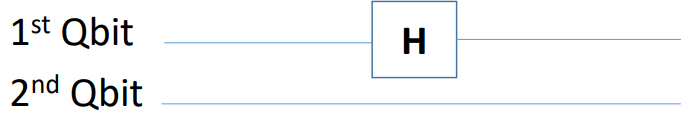
\includegraphics[scale=0.6]{images/circuit_1.PNG}
\end{figure}

\noindent
These circuits are sometimes called \textbf{gates} or \textbf{tensor networks}.
We read circuits from left to right.
The solid lines are \textbf{wires}, corresponding to Qbits.
The boxes correspond to unitary operators.
The CNOT operator is denoted by:

\begin{figure}[h]
    \centering
    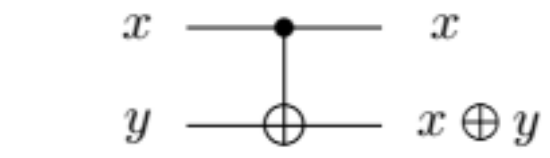
\includegraphics[scale=0.5]{images/cnot.PNG}
\end{figure}

\noindent
Using multiple CNOT gates, we can create a \textbf{SWAP gate}:

\begin{figure}[h]
    \centering
    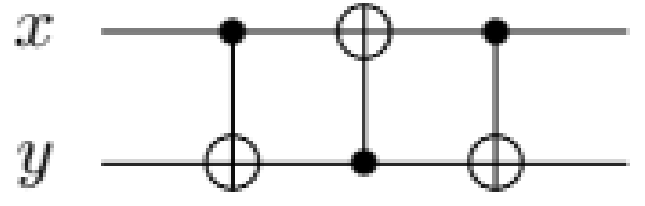
\includegraphics[scale=0.4]{images/swap_gate.PNG}
\end{figure}

\noindent
This gate keeps the states $\ket{00}$ and $\ket{11}$ the same, but swaps the states $\ket{01}$ and $\ket{10}$.

\newpage
\noindent
Generally speaking, all Qbits are initialized to the left of the circuit (usually in $\ket{0}$).
The circuit is then executed from left to right, and usually ends with a measurement on one or more Qbits:

\begin{figure}[h]
    \centering
    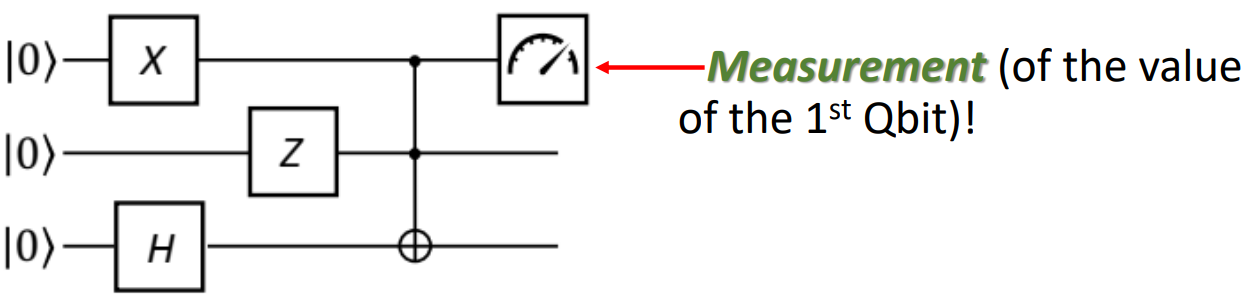
\includegraphics[scale=0.5]{images/measurement_gate.PNG}
\end{figure}

\noindent
A quantum circuit describes the \textbf{evolution} of a quantum system over time (one column = one time step).
Similarly, an appropriate matrix multiplication can describe the same evolution.
Say for example we want to perform a CNOT gate on two non-adjacent Qbits:

\begin{figure}[h]
    \centering
    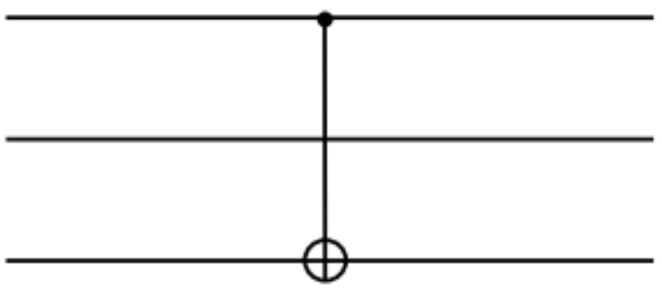
\includegraphics[scale=0.5]{images/non_adjacent_cnot.PNG}
\end{figure}

\noindent
We can do this by swapping the second and third Qbit, applying the CNOT gate, then swapping the second and third Qbit again:

\[ (I_2 \otimes \text{SWAP}) \times (\text{CNOT} \otimes I_2) \times (I_2 \otimes \text{SWAP}) \]

\noindent
We can create every possible quantum circuit by only using the CNOT, H and T (phase transform) gates.
These are called the \textbf{universal gates}.
Additionally, the \textbf{Gottesman-Kill Theorem} states that any quantum circuit consisting only of X, Y, Z, H and CNOT gates can be efficiently simulated on a classical computer.

\subsection*{Bell States}
Two Qbits prepared in the $\ket{0}$ state can be entangled using the following circuit, described in the previous lecture:

\begin{figure}[h]
    \centering
    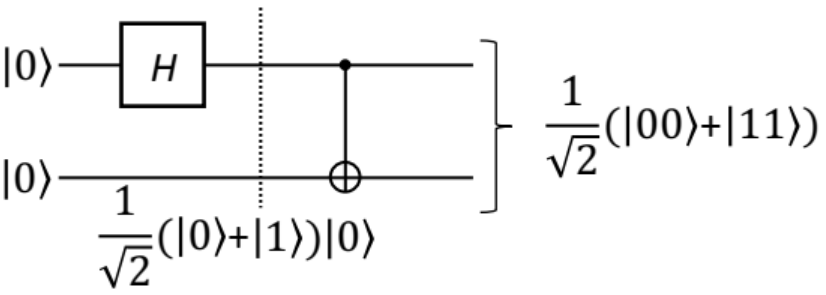
\includegraphics[scale=0.6]{images/bells_state.PNG}
\end{figure}

\newpage
\noindent
There are a total of four different \textbf{Bell states}, each state corresponding to what state we prepare the original Qbits in:

\begin{enumerate}
    \item $\ket{\Phi^+} = \frac{1}{\sqrt{2}}\ket{00} + \frac{1}{\sqrt{2}}\ket{11}$ \hfill $(\ket{0}, \ket{0})$
    \item $\ket{\Psi^+} = \frac{1}{\sqrt{2}}\ket{01} + \frac{1}{\sqrt{2}}\ket{10}$ \hfill $(\ket{0}, \ket{1})$
    \item $\ket{\Phi^-} = \frac{1}{\sqrt{2}}\ket{00} - \frac{1}{\sqrt{2}}\ket{11}$ \hfill $(\ket{1}, \ket{0})$
    \item $\ket{\Psi^-} = \frac{1}{\sqrt{2}}\ket{01} - \frac{1}{\sqrt{2}}\ket{10}$ \hfill $(\ket{1}, \ket{1})$
\end{enumerate}

\noindent
These four states form an orthonormal basis for the 4-dimensional vector space describing composite systems of two Qbits.

%
% Lecture 8 - Quantum Teleportation.
%
\section*{Lecture 8 - Quantum Teleportation}
Given two people, Alice and Bob, the question in this lecture is if Alice can somehow "teleport" the state of her Qbit $\ket{\psi} = \alpha \ket{0} + \beta \ket{1}$ to Bob.
Alice could send Bob the coefficients $\alpha$ and $\beta$, but Alice might not know what these coefficients are (it is not possible to measure $\alpha$ and $\beta$ if you do not know them in advance).

\subsection*{No Cloning Theorem}
Suppose we have a Qbit in some state $\ket{\psi} = \alpha \ket{0} + \beta \ket{1}$, where we do not know what $\alpha$ and $\beta$ are, but we still want to copy this state.
We want to do something to the combined system consisting of $\ket{\psi}$ and another Qbit, for example $\ket{0}$, such that both Qbits end up in the same state $\ket{\psi}$:

\begin{figure}[h]
    \centering
    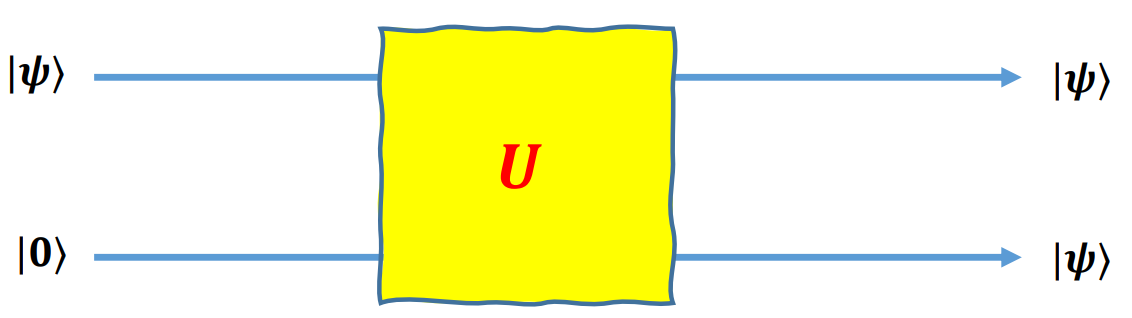
\includegraphics[scale=0.5]{images/no_cloning_theorem.PNG}
\end{figure}

\noindent
The \textbf{No Cloning Theorem} states that there is no such unitary operation $U$ that can copy an arbitrary Qbit state.
If we assume that such a unitary operation $U$ exists, then this quickly leads to a contradiction.

\subsection*{First Approach: Quantum Communication}
Alice wants to send Bob $\ket{\psi} = \alpha \ket{0} + \beta \ket{1}$.
The amplitudes are unknown to Alice.
Assume that Alice and Bob have some means of quantum communication.
In particular, assume that they have a CNOT gate that extends all the way from Alice to Bob.

\newpage
\noindent
Using her unknown Qbit $\ket{\psi}$, Alice applies a CNOT gate to Bob's Qbit.
This means they end up with an entangled state $\alpha \ket{00} + \beta \ket{11}$.
Alice then measures her Qbit in the $\ket{+}, \ket{-}$ basis.
Rewriting the state in this basis, we get:

\[ \alpha \ket{00} + \beta \ket{11} = \alpha \left( \frac{1}{\sqrt{2}}\ket{+} + \frac{1}{\sqrt{2}}\ket{-} \right) \otimes \ket{0} + \beta \left( \frac{1}{\sqrt{2}}\ket{+} - \frac{1}{\sqrt{2}}\ket{-} \right) \otimes \ket{1} \]

\[ \alpha \ket{00} + \beta \ket{11} = \frac{1}{\sqrt{2}}\ket{+}\left( \alpha \ket{0} + \beta \ket{1} \right) + \frac{1}{\sqrt{2}}\ket{-}\left( \alpha \ket{0} - \beta \ket{1} \right) \]

\noindent
If Alice measures $\ket{+}$, then Bob's Qbit will be in the state $\alpha \ket{0} + \beta \ket{1} = \ket{\psi}$.
If Alice measures $\ket{-}$, then Bob's Qbit will be in the state $\alpha \ket{0} - \beta \ket{1}$.
Bob can then apply the $Z$ transformation to his Qbit, which will result in the state $\alpha \ket{0} + \beta \ket{1} = \ket{\psi}$.

\subsection*{Second Approach: Classical Communication}
Alice wants to send Bob $\ket{\psi} = \alpha \ket{0} + \beta \ket{1}$.
The amplitudes are unknown to Alice.
Bob is far away, and they only share a conventional telephone line.

\noindent
\\
What Alice and Bob can do is share an entangled pair of Qbits $\ket{\Phi^+} = \frac{1}{\sqrt{2}}\ket{00} + \frac{1}{\sqrt{2}}\ket{11}$ beforehand.
Alice can then perform some measurement on her unknown Qbit $\ket{\psi}$ and her part of the entangled state $\ket{\Phi^+}$.
If she phones this result to Bob, Bob can then perform one of four possible unitary operations on his part of the entangled state $\ket{\Phi^+}$, which will result in Bob's Qbit being in the state $\ket{\psi}$.
Note that in this process Alice destroys her Qbit $\ket{\psi}$ by measuring it, but we only care about the teleportation to Bob.

\noindent
\\
To be more specific, the composite system of Alice and Bob can be described by:

\[ \left( \alpha \ket{0} + \beta \ket{1} \right) \otimes \ket{\Phi^+} = \frac{\alpha}{\sqrt{2}}\ket{000} + \frac{\alpha}{\sqrt{2}}\ket{011} + \frac{\beta}{\sqrt{2}}\ket{100} + \frac{\beta}{\sqrt{2}}\ket{111} = \ket{\phi} \]

\noindent
Alice then applies a CNOT gate to her two Qbits, with $\ket{\psi}$ being the control bit:

\[ \ket{\phi^\prime} = \frac{\alpha}{\sqrt{2}}\ket{000} + \frac{\alpha}{\sqrt{2}}\ket{011} + \frac{\beta}{\sqrt{2}}\ket{110} + \frac{\beta}{\sqrt{2}}\ket{101} \]

\noindent
If Alice measures the second Qbit (the one from $\ket{\Phi^+}$), then with probability $\frac{1}{2}$ she will see a 0, and with probability $\frac{1}{2}$ she will see a 1.
If she sees a 0, then the new state becomes:

\[ \ket{\phi^\prime} = \alpha \ket{00} + \beta \ket{11} \]

\noindent
If she sees a 1, then the new state becomes:

\[ \ket{\phi^\prime} = \alpha \ket{01} + \beta \ket{10} \]

\noindent
After measuring, Alice phones Bob and tells him if she got a 0 or 1.
If she got a 0, then Bob leaves his Qbit alone, as it is in the desired state already.
If she got a 1, then Bob applies the bit-flip transformation $X$ to his Qbit to get the desired state.

%
% Lecture 9 - Deutsch's Algorithm.
%
\newpage
\section*{Lecture 9 - Deutsch's Algorithm}
With the exceptions of the quantum information protocols we have seen so far, Deutsch's algorithm is historically the first \textbf{quantum algorithm}.
It is also the first computational task that can \textit{provably} be solved faster on a quantum computer.

\noindent
\\
A quantum algorithm is an algorithm that runs on a realistic model of quantum computation, for example the circuit model.
In the circuit model we have a quantum circuit that acts on some input Qbits, and terminates with a measurement on some output Qbits.

\subsection*{Evaluating Boolean Functions}
We are given a boolean function $f:\{ 0, 1 \} \rightarrow \{ 0, 1 \}$ (i.e. $f$ takes as input either 0 or 1, and outputs either 0 or 1).
In total there are four possible boolean functions:

\begin{enumerate}
    \item $f_0(0) = 0, \ f_0(1) = 0 \ $ (constant)
    \item $f_1(0) = 0, \ f_1(1) = 1 \ $ (balanced)
    \item $f_2(0) = 1, \ f_2(1) = 0 \ $ (balanced)
    \item $f_3(0) = 1, \ f_3(1) = 1 \ $ (constant)
\end{enumerate}

\noindent
The question is as follows: given a random boolean function $f$, is $f$ constant or balanced?
To solve this problem classically, we need to plug both 0 and 1 into $f$ and see the result.
It is impossible to solve this problem with less than two queries, unless we have a quantum computer.

\subsection*{Deutsch's Algorithm}
Deutsch's algorithm is given by the following circuit:

\begin{figure}[h]
    \centering
    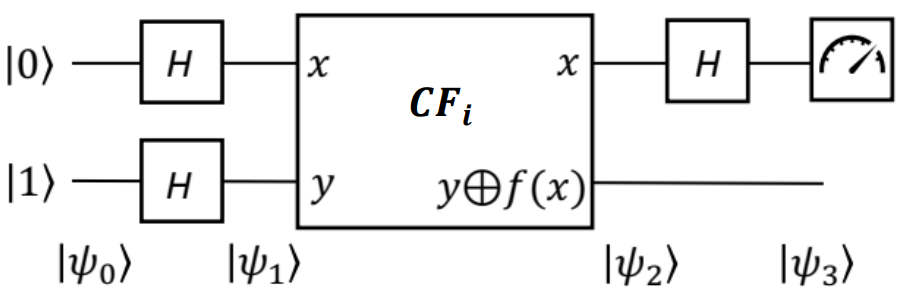
\includegraphics[scale=0.7]{images/deutsch_algorithm.PNG}
\end{figure}

\noindent
Here $CF_i$ is the unknown function $f_i$, $x$ is the input Qbit, $y$ is the control Qbit, and the output is given by $y \oplus f_i(x)$ (where $\oplus$ is an XOR).

\noindent
\\
The initial state is given by $\ket{\psi_0} = \ket{0} \otimes \ket{1} = \ket{01}$.
We pass both Qbits through a Hadamard gate, which puts the state in the following superposition:

\[ \ket{\psi_1} = H(\ket{\psi_0}) = \frac{1}{2}\left( \ket{00} - \ket{01} + \ket{10} - \ket{11} \right) \]

\newpage
\noindent
Next, the two Qbits pass through the $CF_i$ circuit.
This circuit leaves the first Qbit alone, while the second Qbit becomes $\ket{y \oplus f_i(x)}$.
Note that $\ket{x \oplus 0} = \ket{x}$ and $\ket{x \oplus 1}$ flips the value of $x$:

\[ \ket{\psi_2} = \frac{1}{2}\left( \ket{0} \otimes \left( \ket{f_i(0)} - \ket{f_i(0) \oplus 1} \right) + \ket{1} \otimes \left( \ket{f_i(1)} - \ket{f_i(1) \oplus 1} \right) \right) \]

\noindent
Observe that $\ket{f_i(0)} - \ket{f_i(0) \oplus 1}$ is either $\ket{0} - \ket{1}$ or $\ket{1} - \ket{0}$ depending on whether $f_i(0)$ is $\ket{0}$ or $\ket{1}$.
Similarly, $\ket{f_i(1)} - \ket{f_i(1) \oplus 1} = (-1)^{f_i(1)}\left( \ket{0} - \ket{1} \right)$.
With this, we can rewrite $\ket{\psi_2}$ as:

\[ \ket{\psi_2} = \frac{1}{\sqrt{2}}\left( (-1)^{f_i(0)}\ket{0} + (-1)^{f_i(1)}\ket{1} \right) \otimes \frac{1}{\sqrt{2}}\left( \ket{0} - \ket{1} \right) \]

\noindent
This shows that the two Qbits are \textit{not} entangled.
Let us examine the state of the first Qbit for each possible case of $f_i$:

\begin{enumerate}
    \item For $f_0$ we have $f_0(0) = f_0(1) = 0$ and thus $\ket{x} = \frac{1}{\sqrt{2}}\left( \ket{0} + \ket{1} \right)$.
    \item For $f_1$ we have $f_1(0) = 0, f_1(1) = 1$ and thus $\ket{x} = \frac{1}{\sqrt{2}}\left( \ket{0} - \ket{1} \right)$.
    \item For $f_2$ we have $f_2(0) = 1, f_2(1) = 0$ and thus $\ket{x} = \frac{-1}{\sqrt{2}}\left( \ket{0} - \ket{1} \right)$.
    \item For $f_3$ we have $f_3(0) = f_3(1) = 1$ and thus $\ket{x} = \frac{-1}{\sqrt{2}}\left( \ket{0} + \ket{1} \right)$.
\end{enumerate}

\noindent
Next we send this Qbit $\ket{x}$ through another Hadamard gate, which gives us:

\[ \ket{0}, \ \text{if } \ket{x} = \frac{1}{\sqrt{2}}\left( \ket{0} + \ket{1} \right) \]

\[ \ket{1}, \ \text{if } \ket{x} = \frac{1}{\sqrt{2}}\left( \ket{0} - \ket{1} \right) \]

\noindent
If we now measure the Qbit in the standard basis, we will get 0 if $f_i$ is constant, and 1 if $f_i$ is balanced.
And we only had to make one query to $f_i$ to determine if $f_i$ is constant or balanced!

\subsection*{Deutsch-Jozsa Algorithm}
The Deutsch-Jozsa algorithm is a generalization of Deutsch's algorithm.
Instead of having a boolean function $f:\{ 0, 1 \} \rightarrow \{ 0, 1 \}$, we can now deal with \textbf{multivariable functions} $f:\{ 0, 1 \}^n \rightarrow \{ 0, 1 \}$ (i.e. $f$ takes as input $n$ variables that are either 0 or 1, and outputs either 0 or 1).
As before, we want to determine if $f$ is constant (maps all inputs to either 0 or 1) or balanced (maps exactly half of the inputs to 0 and the other half to 1).

\noindent
\\
A similar proof can be constructed for this algorithm, that shows that we only need to make one query to $f$ to determine if $f$ is constant or balanced, as opposed to $2^{n-1} + 1$ queries classically.

\noindent
\\
The circuit for the Deutsch-Jozsa algorithm is given by:

\newpage
\begin{figure}[h]
    \centering
    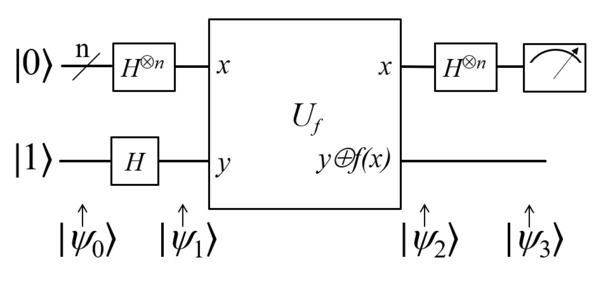
\includegraphics[scale=0.75]{images/deutsch-jozsa_algorithm.PNG}
\end{figure}

\noindent
The diagonal $n$ line means that in reality there are a total of $n$ parallel lines.
The first $n$ Qbits are initialized to $\ket{0}$, and the last Qbit is initialized to $\ket{1}$.
For the first $n$ Qbits, we apply a Hadamard gate to each Qbit.
This operation can be written as $H^{\otimes n}$, which means:

\[ H^{\otimes 2} = \frac{1}{\sqrt{2}} \begin{bmatrix}
    H & H \\
    H & -H
\end{bmatrix}, \ ... \ , \ H^{\otimes n} = \frac{1}{\sqrt{2}} \begin{bmatrix}
    H^{\otimes n - 1} & H^{\otimes n - 1} \\
    H^{\otimes n - 1} & -H^{\otimes n - 1}
\end{bmatrix} \]

\noindent
This gives us an easy way to calculate the composite state of $n$ Qbits that all pass through Hadamard gates.

%
% Lecture 10 - Grover's Algorithm.
%
\section*{Lecture 10 - Grover's Algorithm}
Grover's algorithm (also called \textbf{unordered search}) is a quantum algorithm that finds with high probability a unique key in a database of size $N$.
In terms of an oracle: given a function $f:\{ 0, 1, ... , N - 1 \} \rightarrow \{ 0, 1 \}$ such that $f(x) = 1$ for a single $x$ and $f(y) = 0$ for $\forall y \neq x$, find the key $x$.

\noindent
\\
In classical computing, this would on average take $\frac{N}{2}$ queries to find $x$ find probability $\frac{1}{2}$.
If we assume $N = 2^n$, then this classical algorithm has complexity $O(2^n)$.
Grover's algorithm solves this search problem in $O(\sqrt{N})$, using $O(\log N)$ Qbits and roughly $\sqrt{N}\log N$ quantum gates.

\subsection*{First Steps}
We need to find a unique solution $x^\prime$, such that $f(x^\prime) = 1$ and $f(x)_{x \neq x^\prime} = 0$.
Assume $N = 2^n$ for some positive integer $n$.

\noindent
\\
Prepare $n$ Qbits in the state $\ket{0}^{\otimes n}$.
At this point, each $x$ has an equal possibility to be the solution $x^\prime$.
We can describe this lack of information by applying a Hadamard gate to each Qbit, which produces an equal superposition of all possible $n$-Qbit strings $x$:

\[ H^{\otimes n} \ket{0}^{\otimes n} = \frac{1}{2^{\frac{n}{2}}} \sum_{x \in \{ 0, 1 \}^n} \ket{x} = \ket{\Psi} \]

\noindent
If we measure this state, we will get an equally random $x$.

\newpage
\noindent
Assume we have access to the oracle function $f$, as described above.
We can now define a unitary operator $U_f$ that acts on the $n$ Qbits and a control bit $\ket{\alpha}$ as follows:

\[ \ket{x} \otimes \ket{\alpha} \stackrel{U_f}{=} \ket{x} \otimes \ket{\alpha \oplus f(x)} \]

\begin{itemize}
    \item If $\ket{\alpha} = \ket{0}$ we get $\ket{x} \otimes \ket{f(x)}$.
    \item If $\ket{\alpha} = \ket{1}$ we get $\ket{x} \otimes \ket{1 \oplus f(x)}$ (flips $f(x)$).
    \item If $\ket{\alpha} = \ket{-} = \frac{1}{\sqrt{2}}(\ket{0} - \ket{1})$ we get $\ket{x} \otimes \left( \frac{1}{\sqrt{2}}\ket{f(x)} - \frac{1}{\sqrt{2}}\ket{1 \oplus f(x)} \right) = (-1)^{f(x)}\ket{x}$.
\end{itemize}

\noindent
This gives us:

\[ U_f(\ket{x} \otimes \ket{-}) = (-1)^{f(x)}\ket{x} = \left\{ \begin{array}{rl}
     \ket{x} & \text{if } f(x) = 0 \\
    -\ket{x} & \text{if } f(x) = 1 \rightarrow x = x^\prime
\end{array} \right. \]

\noindent
This oracle $U_f$ flips the amplitude of the solution $x^\prime$, while all the other amplitudes remain unchanged:

\begin{figure}[h]
    \centering
    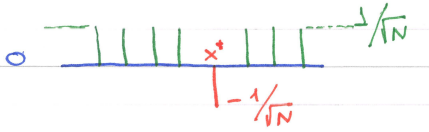
\includegraphics{images/grovers_step_1.PNG}
\end{figure}

\subsection*{Inversion About the Mean}
Let $\mu = \sum_{x} \frac{\alpha_x}{N}$ be the mean of the amplitudes $\alpha_x$ for all $x$.
The inversion of $\alpha_{x^\prime}$ lowers the mean by a small amount.

\noindent
\\
We can define a new (unitary) operation that flips each amplitude $\alpha_x$ about the mean $\mu$:

\[ \alpha_x = 2\mu - \alpha_x \]

\noindent
After the phase inversion followed by the inversion about the mean, the amplitude of $x^\prime$ becomes:

\[ \frac{1}{\sqrt{N}} \ \stackrel{\text{phase inversion}}{\longrightarrow} \ \frac{-1}{\sqrt{N}} \ \stackrel{\text{inversion about the mean}}{\longrightarrow} \ 2\mu - \left(\frac{-1}{\sqrt{N}}\right) = 2 \cdot \frac{1}{\sqrt{N}} + \frac{1}{\sqrt{N}} = \frac{3}{\sqrt{N}} \]

\noindent
This shows we have amplified the amplitude of $x^\prime$ by $\frac{2}{\sqrt{N}}$.
If we repeat this process (phase inversion followed by inversion about the mean), the amplitude of $x^\prime$ will be further increased to $\frac{5}{\sqrt{N}}$, then $\frac{9}{\sqrt{N}}$, etc.
After roughly $\sqrt{\frac{N}{2}}$ iterations, the amplitude of $x^\prime$ will be $\frac{1}{\sqrt{2}}$.
This means that if we perform a measurement, we will observe $x^\prime$ with probability $\frac{1}{2}$.

\newpage
\subsection*{Implementing Inversion About the Mean}
It turns out that inversion about the mean is the same as doing a reflection about the uniform superposition $\ket{u} = \frac{1}{\sqrt{N}} \sum_x \ket{x}$.
One way to perform such a reflection is as follows:

\begin{enumerate}
    \item Transform $\ket{u}$ to $\ket{0}^{\otimes n}$.
    \item Do a reflection about $\ket{0}^{\otimes n}$.
    \item Transform back to $\ket{u}$.
\end{enumerate}

\noindent
Note that all of these steps are unitary.
For the first step, we can apply $H^{\otimes n}$ to $\ket{u}$.
For the second step, we need to reflect about $\ket{0}^{\otimes n}$.
This can be done by multiplying all vectors in the orthogonal subspace of $\ket{0}^{\otimes n}$ by -1:

\[ \begin{bmatrix}
    1 & 0 & ... & 0 \\
    0 & -1 & ... & 0 \\
    \vdots & \vdots & \ddots & \vdots \\
    0 & 0 & ... & -1
\end{bmatrix} = 2\ket{0}\bra{0} - I \] 

\noindent
Note that the first diagonal element is 1, since $\ket{0}\bra{0}$ creates an empty matrix with a 1 in the top-left corner.
For the third step, we need to apply $H^{\otimes n}$ again ($H$ is its own inverse).
This whole procedure can be written as:

\[ H^{\otimes n} (2\ket{0}\bra{0} - I) H^{\otimes n} = 2\ket{u}\bra{u} - I \]

\noindent
This is called the \textbf{reflection / diffusion operator}: given a vector $\ket{\alpha}$, the unitary operator $2\ket{\alpha}\bra{\alpha} - I$ performs a reflection about $\ket{\alpha}$.
Identically, the unitary operator $I - 2\ket{\alpha}\bra{\alpha}$ performs a reflection about $\ket{\alpha^\perp}$: the orthogonal subspace of $\ket{\alpha}$.
Following this, the phase inversion operator shown earlier is actually a rotation about $\ket{\Psi}$.
This is called the \textbf{phase shift operator}.

\subsection*{Geometric Interpretation}
The first step in Grover's algorithm is to reflect $\ket{u} = \frac{1}{\sqrt{2^n}} \sum_x \ket{x}$ about $\ket{\Psi} = \frac{1}{\sqrt{2^n - 1}} \sum_{x \neq x^\prime} \ket{x}$.
This gives us the following state:

\[ \ket{\alpha_1} = \cos \theta \ket{\psi} - \sin \theta \ket{x^\prime} \]

\noindent
With $\sin \theta = \frac{1}{\sqrt{2^n}}$ and $\cos \theta = \sqrt{\frac{2^n - 1}{2^n}}$.
In general, if we have $N$ elements and $M$ solutions, then:

\[ \sin \theta = \sqrt{\frac{M}{N}}, \ \cos \theta = \sqrt{\frac{N - M}{N}} \]

\noindent
The next step is to apply inversion about the mean to $\ket{\alpha_1}$, which produces the following state:

\[ \ket{\alpha_2} = \cos 3\theta \ket{\psi} - \sin 3\theta \ket{x^\prime} \]

\noindent
If we apply this process $k$ times, we get the following state:

\[ \ket{\alpha_k} = \cos (2k + 1) \theta \ket{\psi} - \sin (2k + 1) \theta \ket{x^\prime} \]

%
% Lecture 11 - Simon's Algorithm.
%
\newpage
\section*{Lecture 11 - Simon's Algorithm}
Let $f: \{ 0, 1 \}^n \rightarrow \{ 0, 1 \}^n$, i.e. $f$ takes as input $n$-bit strings and outputs $n$-bit strings.
$f$ has the property that $f(x) = f(y)$ if and only if $x = y$ or $x = y \oplus s$ for some $n$-bit string $s \neq 0^n$.
\textbf{Simon's problem} is to find $s$ with as few queries to $f$ as possible.

\noindent
\\
An interesting property of $f$ is that $f$ is \textbf{periodic}, i.e. if $f(a) = f(b)$ then $f(b) = f(a)$ for all possible strings $a, b \in \{ 0, 1 \}^n$.
This means that, classically, we can find the solution $s$ in at most $2^{n - 1} + 1$ queries to $f$.
For example with $n = 3$, we can query $f(000), f(001), f(010)$ and $f(011)$ without getting any collisions, but when we query $f(100)$, we must get a collision with one of the previous queries.
Once we have a collision, we can easily reverse engineer $s = a \oplus b$, where $a$ and $b$ are the strings that collided.

\noindent
\\
To improve this algorithm, we first need to understand the \textbf{dot product} of two binary strings:
\[ a \cdot b = a_0b_0 \oplus a_1b_1 \oplus ... \oplus a_{n-1}b_{n-1} \]

\noindent
This determines if two binary strings differ in an odd (0) or even (1) number of positions.

\subsection*{Simon's Circuit}
Given the black box operator $U_f$, Simon constructed the following circuit:

\begin{figure}[h]
    \centering
    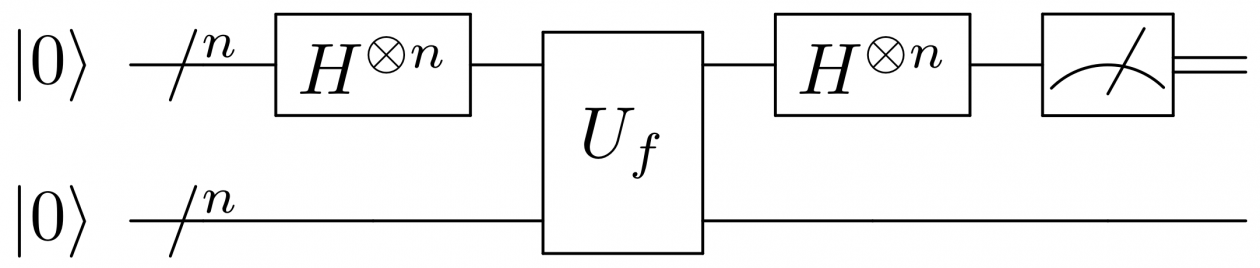
\includegraphics[scale=0.4]{images/simons_circuit.png}
\end{figure}

\noindent
For easiness, we will work with $n = 2$.

\noindent
\\
\textbf{Step 1:} The first input passes through a Hadamard gate:

\[ \ket{00} \rightarrow \frac{1}{2}\left( \ket{00} + \ket{01} + \ket{10} + \ket{11} \right) \]

\noindent
The second input remains unchanged.
The composite state after this step is:
\[ \frac{1}{2}\left( \ket{00} + \ket{01} + \ket{10} + \ket{11} \right) \otimes \ket{00} = \frac{1}{2}\left( \ket{00} \otimes \ket{00} + \ket{01} \otimes \ket{00} + \ket{10} \otimes \ket{00} + \ket{11} \otimes \ket{00} \right) \]

\noindent
\textbf{Step 2:} Now the Qbits pass through the black box operator $U_f$.
The new composite state is:

\[ \frac{1}{2}\left( \ket{00} \otimes \ket{f(00)} + \ket{01} \otimes \ket{f(01)} + \ket{10} \otimes \ket{f(10)} + \ket{11} \otimes \ket{f(11)} \right) \]

\noindent
This is because $\ket{y_0 ... y_{n - 1}} = \ket{0 ... 0}$ and $\ket{0 ... 0} \oplus \ket{f(x_0 ... x_{n - 1})} = \ket{f(x_0 ... x_{n - 1})}$.

\noindent
\\
\textbf{Step 3:} The top Qbits pass through another Hadamard gate.
The new composite state is:

\newpage

\begin{table}[h]
    \centering
    \begin{tabular}{lllll}
    $\frac{1}{4}\left( \ket{00} + \ket{01} + \ket{10} + \ket{11} \right)$ & $\otimes$ & $\ket{f(00)}$ & $+$ &  \\
    $\frac{1}{4}\left( \ket{00} - \ket{01} + \ket{10} - \ket{11} \right)$ & $\otimes$ & $\ket{f(01)}$ & $+$ &  \\
    $\frac{1}{4}\left( \ket{00} + \ket{01} - \ket{10} - \ket{11} \right)$ & $\otimes$ & $\ket{f(10)}$ & $+$ &  \\
    $\frac{1}{4}\left( \ket{00} - \ket{01} - \ket{10} + \ket{11} \right)$ & $\otimes$ & $\ket{f(11)}$ & $=$ & $\ket{\Phi}$
    \end{tabular}
\end{table}

\noindent
We can rearrange this with respect to $\ket{00}, ... , \ket{11}$:

\begin{table}[h]
    \centering
    \begin{tabular}{lllll}
    $\frac{1}{4}\ket{00}$ & $\otimes$ & $\left( \ket{f(00)} + \ket{f(01)} + \ket{f(10)} + \ket{f(11)} \right)$ & $+$ &  \\
    $\frac{1}{4}\ket{01}$ & $\otimes$ & $\left( \ket{f(00)} - \ket{f(01)} + \ket{f(10)} - \ket{f(11)} \right)$ & $+$ &  \\
    $\frac{1}{4}\ket{10}$ & $\otimes$ & $\left( \ket{f(00)} + \ket{f(01)} - \ket{f(10)} - \ket{f(11)} \right)$ & $+$ &  \\
    $\frac{1}{4}\ket{11}$ & $\otimes$ & $\left( \ket{f(00)} - \ket{f(01)} - \ket{f(10)} + \ket{f(11)} \right)$ & $=$ & $\ket{\Phi}$ \\
    \end{tabular}
\end{table}

\noindent
\textbf{Step 4:} We now measure the top Qbits.
We know that, no matter what, the dot product between the measurement outcome and the solution $s$ will be 0 (proof omitted).
Using this, we can find that each possible measurement outcome corresponds to a single Qbit of $s$.
This means that, to find $s$, we need to perform this entire circuit an expected $n - 1$ times to get the solution $s$ (not $n$ times since $s \neq 0^n$).
This shows us that we can solve Simon's problem \textbf{exponentially faster} using a quantum computer.

%
% Lecture 12 - Quantum Cryptography.
%
\section*{Lecture 12 - Quantum Cryptography}
\subsection*{Shor's Algorithm}
Shor's algorithm concerns the Integer Factorization Problem, for which no known classical algorithm can solve it in polynomial time.
The problem is as follows: given an integer $N$, find its \textbf{prime factors} $p$ and $q$.
A classical way to solve this is to try all possible divisors up to $\sqrt{N}$, which takes exponential time.
Shor's algorithm solves this problem on a quantum computer in $O\left( \left( \log N \right)^3 \right)$ time.

\noindent
\\
To solve the Integer Factorization Problem, we need to find the smallest $r$ such that $f(x) = f(x + r)$ for the following $f$:
\[ f(x) = a^x \ mod \ N \]

\noindent
Where $a$ is some initial guess for a factor of $N$.
If we know $r$, then with a high probability one of $a^{\frac{r}{2}} + 1$ or $a^{\frac{r}{2}} - 1$ is a prime factor of $N$.
If this is not the case, then we use one of these values as a new $a$ and try again.
We can find $r$ efficiently using the \textbf{Quantum Fourier Transform}.

\noindent
\\
The reason this algorithm is a big deal is because it can break the \textbf{RSA Cryptography System}, which depends on the factorization of large integers.
Even though quantum computers are currently not powerful enough to break RSA, we should still start looking for new cryptography systems that are \textbf{quantum-safe}.

\subsection*{BB84 Protocol}
The BB84 protocol is a \textbf{quantum key distribution} scheme.
It is the first quantum cryptography protocol that was proven to be \textbf{unconditionally secure}.
It requires a classical channel as well as a quantum channel of communication between two parties (Alice and Bob).

\newpage
\noindent
For Alice and Bob to be able to communicate securely, they will need to share a secret key that only they know.
Alice takes some binary string (e.g. 01010101), encodes each bit either in the $\{ \ket{0}, \ket{1} \}$ basis or the $\{ \ket{+}, \ket{-} \}$ basis at random, and sends the resulting bits to Bob through the quantum channel.

\noindent
\\
Bob receives the Qbits, and measures each Qbit in either the $\{ \ket{0}, \ket{1} \}$ basis or the $\{ \ket{+}, \ket{-} \}$ basis at random.
He then shares with Alice (using a non-secure channel) in which basis he measured each Qbit.
Alice then tells Bob which of his measurements were correct, and which were incorrect.
If Bob was correct, then he keeps the bit and appends it to the key.
Otherwise, he discards the bit.
At the end, Alice and Bob will have a shared key that only they know.

\noindent
\\
If an eavesdropper (Eve) tries to intercept the Qbits, she will have to measure each Qbit in either the $\{ \ket{0}, \ket{1} \}$ basis or the $\{ \ket{+}, \ket{-} \}$ basis at random.
But since she \textit{measures} each Qbit, she will corrupt it, and Alice and Bob will notice that some of their measurements are incorrect.
Not only is Eve unable to get the key, but Alice and Bob will know that Eve tried to intercept their communication.
This means that the BB84 protocol is \textbf{unconditionally secure}.

\end{document}
